\documentclass{article}
\usepackage[spanish]{babel}
\usepackage[utf8x]{inputenc}
\usepackage{graphicx}
% \usepackage{epstopdf}
% \epstopdfsetup{outdir=./}
\usepackage{subfigure}
\usepackage{hyperref}
% \usepackage{mathpazo}
\usepackage{amsmath}
\usepackage{amssymb}
\usepackage{ textcomp }
\usepackage{booktabs}
\usepackage[inline]{enumitem}
\hypersetup{colorlinks=true,citecolor=black,filecolor=black,linkcolor=black,urlcolor=black}

% package for bibliography
% \usepackage[authoryear,round]{natbib}

\usepackage{amsmath}
\usepackage{amsfonts}
\usepackage{algorithm}
\usepackage{algorithmic}
\floatname{algorithm}{Algoritmo}
\renewcommand{\listalgorithmname}{Lista de algoritmos}
\renewcommand{\algorithmicrequire}{\textbf{Entrada:}}
\renewcommand{\algorithmicensure}{\textbf{Salida:}}
\renewcommand{\algorithmicend}{\textbf{fin}}
\renewcommand{\algorithmicif}{\textbf{si}}
\renewcommand{\algorithmicthen}{\textbf{entonces}}
\renewcommand{\algorithmicelse}{\textbf{si no}}
\renewcommand{\algorithmicelsif}{\algorithmicelse,\ \algorithmicif}
\renewcommand{\algorithmicendif}{\algorithmicend\ \algorithmicif}
\renewcommand{\algorithmicfor}{\textbf{para}}
\renewcommand{\algorithmicforall}{\textbf{para todo}}
\renewcommand{\algorithmicdo}{\textbf{hacer}}
\renewcommand{\algorithmicendfor}{\algorithmicend\ \algorithmicfor}
\renewcommand{\algorithmicwhile}{\textbf{mientras}}
\renewcommand{\algorithmicendwhile}{\algorithmicend\ \algorithmicwhile}
\renewcommand{\algorithmicloop}{\textbf{repetir}}
\renewcommand{\algorithmicendloop}{\algorithmicend\ \algorithmicloop}
\renewcommand{\algorithmicrepeat}{\textbf{repetir}}
\renewcommand{\algorithmicuntil}{\textbf{hasta que}}
\renewcommand{\algorithmicprint}{\textbf{imprimir}} 
\renewcommand{\algorithmicreturn}{\textbf{devolver}} 
\renewcommand{\algorithmictrue}{\textbf{cierto }} 
\renewcommand{\algorithmicfalse}{\textbf{falso }} 


\begin{document}
\title{
	\begin{figure}[!ht]
	\centering
		
\includegraphics[scale=0.8]{resources/images/cinvestav-logo}
		\\[0.5cm]LTI Cinvestav Tamaulipas
	\end{figure}
	\vspace{1cm}
	Técnicas de validación y remuestreo{\small[1.e.ii-v]}
	\vspace{1cm}
}
	
\author{Rafael Pérez Torres}	
		
\date{
	Tópicos Selectos en Reconocimiento de Patrones \\ 
	\vspace{0.8cm}
	Profesor Dr. Wilfrido Gómez Flores \\
	\vspace{1cm}
	%\today
}

\maketitle
% \setlength{\parindent}{0pt}

\begin{abstract}
Resumen
\end{abstract}

\section{Introducción}
Los métodos de remuestreo y validación cruzada resultan útiles para dos tareas en particular, la selección del modelo y la estimación del performance de los clasificadores.

En el caso de la selección del modelo, es importante destacar que todas las técnicas de clasificación cuentan con uno o más parámetros que deben ser adaptados.
Por ejemplo, el número de vecinos en un clasificador k-nn o el tamaño de la red, parámetros de aprendizaje y pesos en una red neuronal.
¿Cómo poder adaptar dichos parámetros?
En el caso de la estimación del performance, es importante destacar que dicha medida debería ser realizada cuando se aplica el clasificador a la población total.
¿Cómo estimar dicho performance?

Si se tuviera acceso a un número ilimitado de muestras, ambas preguntas tendrían una respuesta inmediata: bastaría elegir el modelo que provea la tasa de error más baja en la población completa, y que dicha tasa de error sea igual al valor verdadero.
Sin embargo, en el mundo real solamente se tiene acceso a un conjunto finito de muestras que es usualmente menor a la cantidad que se desearñia.
Un enfoque aplicable sería utilizar el conjunto de datos completo para seleccionar al clasificador y estimar el error. Sin embargo, este enfoque tiene dos problemas fundamentales:
\begin{itemize}
	\item El modelo final estaría sobreentrenado, lo cual se hace evidente en modelos con un número grande de parámetros. En la práctica el clasificador fallaría al asignar las etiquetas a las muestras que \emph{no vio} durante la etapa de entrenamiento.
	\item El error estimado sería marcadamente optimista (menor que el error real).
\end{itemize}


En general, las técnicas de remuestreo y validación cruzada intentar dar respuesta a este problema a través de mecanismos para realizar la división del conjunto de  datos.
Por un lado, las técnicas de validación cruzada dividen el conjunto de datos en partes que son independientes una de las otras; en otras palabras, no existen elementos repetidos en cada una de dichas partes.
Por otro lado, las técnicas de remuestreo permiten crear particiones en las que los elementos son seleccionados \emph{con reemplazo}, pudiendo aparecer más de una ocasión tanto en el conjunto de entrenamiento como en el de prueba.

El sobreentrenamiento o sobre-ajuste ocurre cuando el tamaño de los datos de entrenamiento es sumamente pequeño o cuando el número de parámetros del modelo es grande, y en general se refiere al hecho de que el clasificador es incapaz de reconocer correctamente muestras que \emph{no haya visto} durante la etapa de entrenamiento.

En base a las particularidades de la división del conjunto de datos, es posible estimar la magnitud del error a obtener por el clasificador.
Habitualmente, la selección de los conjuntos y el entrenamiento y clasificación asociados, se realiza en varias intervenciones, obteniendo la media de los resultados como el valor final del error.
% Un aspecto interesante de las distintas técnicas de validación cruzada y remuestreo es la posibilidad de evaluar la precisión de los resultados que los clasificadores obtendrían al utilizarlas.

% Un inductor (\textbf{inducer}) o algoritmo de inducción crea un clasificador a partir de un dataset.
% Sea $\mathcal{V}$ el espacio de instancias no etiquetadas y $\mathcal{Y}$ el conjunto de etiquetas disponibles.
% Sea $\mathcal{X} = \mathcal{V} \times \mathcal{Y}$  el espacio de instancias etiquetadas y $\mathcal{D} = \left \{ x_1,x_2,\ldots,x_n \right \}$ un dataset con $n$ instancias etiquetadas, donde $x_i = \langle v_i \in \mathcal{V}, y_i \in \mathcal{Y} \rangle$.
% Un clasificador $\mathcal{C}$ mapea una instancia no-etiquetada $v \in \mathcal{V}$ hacia una etiqueta $y \in \mathcal{Y}$ y un inductor $\mathcal{I}$ mapea un dataset $\mathcal{D}$ en un clasificador $\mathcal{C}$.
% La notación $\mathcal{I}(\mathcal{D},v)$ denota la etiqueta asignada a una instancia $v$ no etiquetada por el clasificador construido por el inductor $\mathcal{I}$ en el dataset $\mathcal{D}$, por ejemplo $\mathcal{I}(\mathcal{D},v) = (\mathcal{I}(\mathcal{D}))(v)$.

% La precisión \textbf{accuracy} de un clasificador $\mathcal{C}$ es la probabilidad de clasificar correctamente una instancia seleccionada aleatoriamente, denotado como $acc = Pr(\mathcal{C}(v) = y)$ para una instancia $\langle v, y \rangle \in \mathcal{X}$.

% La medición de la precisión de un clasificador, normalmente es realizada a partir de la media de $n$ ejecuciones del mismo.

\section{Técnicas de validación cruzada}
% In cross validation we randomly split the set of labeled training samples D into two
% parts: one is used as the traditional training set for adjusting model parameters in the
% classifier. The other set — the validation set — is used to estimate the generalization validation
% set error. Since our ultimate goal is low generalization error, we train the classifier until
% we reach a minimum of this validation error, as sketched in Fig. 9.9. It is essential that
% the validation (or the test) set not include points used for training the parameters in
% the classifier — a methodological error known as “testing on the training set.” 

% Cross validation can be applied to virtually every classification method, where the
% specific form of learning or parameter adjustment depends upon the general training method. For example, in neural networks of a fixed topology (Chap. ??), the amount
% of training is the number of epochs or presentations of the training set. Alternatively,
% the number of hidden units can be set via cross validation. Likewise, the width of the
% Gaussian window in Parzen windows (Chap. ??), and an optimal value of k in the

Las técnicas de validación cruzada básicamente dividen al conjunto de datos, de tal manera que cada una de las particiones contienen elementos únicos y cada elemento puede aparecer únicamente en una sola partición.
La división es aleatoria obteniendo dos conjuntos, uno que se utiliza como el clásico conjunto de entrenamiento, y el otro -- de validación -- es utilizado para estimar el error de generalización del conjunto de validación.
Dado que el objetivo final en el diseño de un clasificador es alcanzar un error bajo de generalización, se entrena al clasificador hasta que se obtiene un valor mínimo de este error.
La validación cruzada puede ser aplicada a virtualmente cada método de clasificación, con la salvedad de adaptar el método de validación a las particularidades de cada técnica.

\begin{figure}
	\centering
	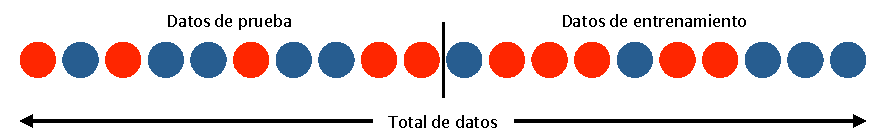
\includegraphics[width=\textwidth]{resources/images/validacion-cruzada-general}
	\caption{División básica de los métodos de validación cruzada}
	\label{fig:validacion-cruzada-general}
\end{figure}

En general, la validación cruzada sólo produce resultados significativos si el conjunto de validación y prueba de conjunto se han extraído de la misma población.
Las siguientes son las técnicas de validación cruzada más utilizadas.


\subsection{Hold out validation}
El método holdout, algunas veces llamado estimación de muestra de prueba, divide a los datos en dos subconjuntos mutuamente exclusivos, denominados conjunto de entrenamiento y conjunto de prueba (o conjunto holdout).
Comúnmente, se designa $2/3$ del conjunto de datos para el entrenamiento y el $1/3$ restante para estimar el error del clasificador entrenado, como se muestre en la Figura~\ref{fig:holdout-validation}.
\begin{figure}
	\centering
	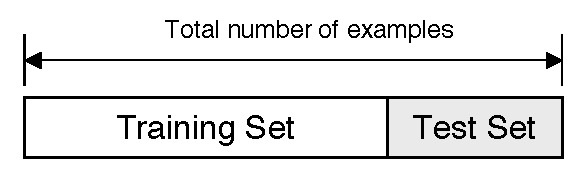
\includegraphics[width=0.5\textwidth]{resources/images/holdout}
	\caption{Holdout validation}
	\label{fig:holdout-validation}
\end{figure}


Las principales desventajas del método holdout son referentes a que no en todos los problemas se cuenta con una cantidad suficiente de instancias para poder aislar un subconjunto especial para la prueba.
Además, dado que su naturaleza es de un sólo experimento de entrenamiento y prueba, la estimación del error tiende a ser no representativa.
% El conjunto de prueba es proporcionado al inductor, mientras que el clasificador obtenido es probado con el conjunto de prueba.
% Formalmente, sea $\mathcal{D}_h$, el conjunto holdout, un subconjunto de $\mathcal{D}$ de tamaño $h$, y sea $\mathcal{D}_t$ como $\mathcal{D} \setminus \mathcal{D}_h$. 
% La estimación de la precisión del método holdout se define como:
% $$
% \text{acc}_h = \frac{1}{h} \sum_{\langle v_i,y_i \rangle \in \mathcal{D}_h} \delta \left \{ \mathcal{I}(\mathcal{D}_t,v_i), y_i \right \}
% $$ % 
% donde $\delta(i,j) = 1$ si $i = j$ y $0$ de otra forma.
En última instancia, la técnica holdout hace un uso ineficiente de los datos, ya que casi un tercio del dataset no es utilizado para entrenar el clasificador~\cite{RonKohavi}.
La mayor cantidad de instancias destinadas al conjunto de prueba incrementan el bias de la estimación.


\subsection{K-­fold cross validation}
En la validación cruzada K-fold, también llamada estimación de rotación, el conjunto de datos se divide aleatoriamente en $k$ particiones mutuamente excluyentes.
La ejecución del clasificador es realizada $k$ veces en los tiempos $t \in \left \{ 1,2,\ldots,k \right \} $.
Por cada experimento realizado en el tiempo $t$, se utilizan $k-1$ particiones para el entrenamiento y la restante se destina para la prueba, como se muestra en la Figura~\ref{fig:k-fold}
\begin{figure}
	\centering
	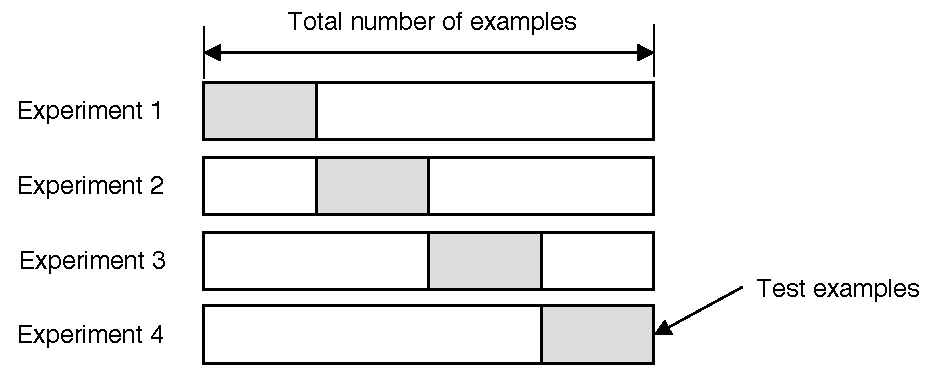
\includegraphics[width=0.5]{resources/images/k-fold}
	\caption{K-fold cross validation}
	\label{fig:k-fold}
\end{figure}

La principal ventaja de la validación cruzada k-fold es que todos los ejemplos del dataset son eventuelmente utilizados para entrenamieto y prueba.
El error real puede ser estimado como el error promedio:
$$
	E = \frac{1}{k} \sum_{i=1}^k E_{i}
$$

\subsubsection*{Cuántas particiones se necesitan?}
Un número grande de particiones arrojaría los siguientes resultados:
\begin{itemize}
	\item \checkmark El bias del estimador del error real sería pequeño.
	\item \texttimes La varianza del estimador del error real sería grande.
	\item \texttimes El tiempo de cómputo sería muy grande (muchos experimentos).
\end{itemize}

Un número pequeño de particiones obtendría:
\begin{itemize}
	\item \checkmark El número de experimentos y tiempo computacional sería reducido.
	\item \checkmark La varianza del estimador del error real sería pequeña.
	\item \texttimes El bias del estimador sería grande
\end{itemize}

En la práctica, la elección del número de particiones depende del tamaño del dataset.
Para datasets grandes, incluso 3-fold cross validation sería preciso.
Para datasets dispersos, es aconsejable utilizar leave-one-out para entrenar con la mayor cantidad de ejemplos posibles. Una elección comúm para k-fold cross validation es $k=10$.

% En la validación cruzada K--fold, también llamada estimación de rotación, el conjunto de datos $\mathcal{D}$ es dividido de forma aleatoria en $k$ subconjuntos mutuamente excluyentes, los \emph{folds}, $\mathcal{D}_1, \mathcal{D}_2, \ldots \mathcal{D}_k$ de un mismo tamaño (o aproximado).
% El inductor es entrenado $k$ veces; cada tiempo $t \in \left \{ 1,2,\ldots,k \right \} $, éste se entrena en $\mathcal{D} \setminus \mathcal{D}_t$ y se prueba sobre $\mathcal{D}_t$.
% La estimación de precisión de la validación cruzada es la cantidad total de clasificaciones correctas, dividida por el número de instancias del data set.
% Formalmente, sea $\mathcal{D}_{(i)}$ el conjunto de prueba que incluye instancias $x_i \langle v_i, y_i \rangle$, entonces la precisión es
% $$
% \text{acc}_{cv} = \frac{1}{n} \sum_{\langle v_i, y_i \rangle \in \mathcal{D} } \delta \left \{ \mathcal{I}(\mathcal{D} \setminus \mathcal{D}_{(i)}, v_i), y_i \right \}
% $$ 
\subsection{Leave-­one-out cross validation (LOOCV)}
Es un caso especial de k-fold cross validation, cuando se indica que K sea el número total de ejemplos.
Para un dataset de $n$ muestras, se desarrollan $n$ experimentos.
En cada experimento, se utilizan entonces $n-1$ instancias para entrenamiento y la restante para la prueba, tal como se muestra en la Figura 
Esta validación cruzada indica separar los datos de tal forma que se tenga una sola muestra para el subconjunto de de prueba y el resto de datos para el subconjunto de entrenamiento, tal como se muestra en la Figura~\ref{fig:leave-one-out-validation}.
\begin{figure}
	\centering
	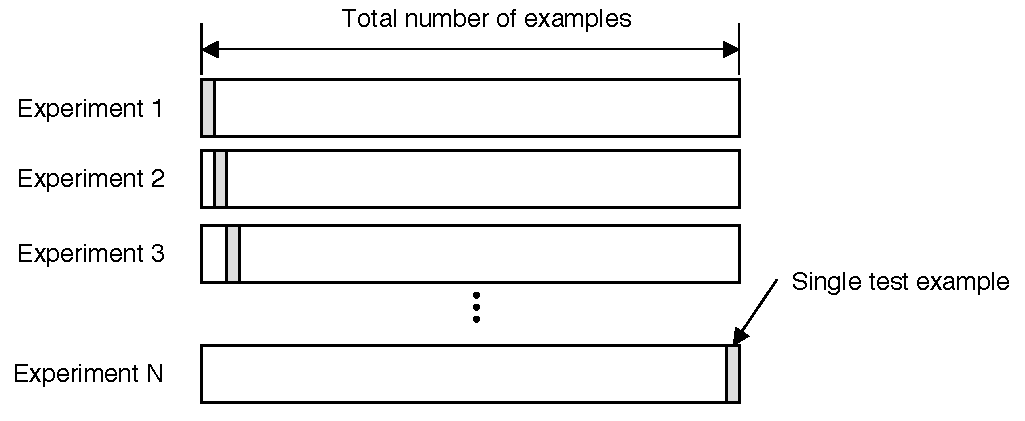
\includegraphics[width=0.5]{resources/images/leave-one-out}
	\caption{Leave-one-out cross validation}
	\label{fig:leave-one-out-validation}
\end{figure}

El error real puede ser estimado como el error promedio obtenido en los ejemplos de prueba:
$$
	E = \frac{1}{n} \sum_{i=1}^n E_{i}
$$


\section{Bootstrap, Bootstrap .632 y Bootstrap .632+}

\section{División de datos en tres conjuntos}
Normalmente, si la selección del modelo y las estimaciones del error real van a ser calculadas simultáneamente, los datos necesitan ser divididos en tres conjuntos disjuntos.
\begin{itemize}
	\item \textbf{Entrenamiento}: Un conjunto de ejemplos utilizados para aprendizaje, en específico para ajustar los parámetros del clasificador.
	\item \textbf{Validación}: Un conjunto de instancias utilizadas para adaptar los parámetros del clasificador.
	\item \textbf{Prueba}: Un conjunto de ejemplos utilizados únicamente para evaluar el desempeño de un clasificador compltamente entrenado. Después de esta evaluación, el modelo ya no debe ser modificado.
\end{itemize}

El procedimiento para su ejecución es mostrado en el Algoritmo~\ref{alg:algoritmo}. 
Dicho algoritmo asume un métdo holdout, en caso de utilizar validación cruzada o bootstrap, los pasos 3 y 4 deben ser repetidos por cada una de las $k$ particiones. 

\begin{algorithm} 
\begin{algorithmic}[1] 
\STATE Dividir el conjunto de datos disponible en subconjuntos de entrenamiento, validación y prueba.
\STATE Seleccionar una arquitectura de clasificador y parámetros de entrenamiento. \label{paso-2}
\STATE Entrenar el modelo a través del conjunto de entrenamiento. 
\STATE Evaluar el modelo utilizando el conjunto de validación. \label{paso-4}
\STATE Repetir los pasos \ref{paso-2} al \label{paso-4} utilizando distintas arquitecturas y parámetros de entrenamiento.
\STATE Seleccionar el mejor modelo y entrenarlo utilizando los datos de los conjuntos de entrenamiento y validación.
\STATE Evaluar el desempeño de este modelo final utilizando el conjunto de prueba.
\end{algorithmic} 
\caption{Algoritmo para realizar entrenamiento, validación y prueba de un clasificador} 
\label{alg:algoritmo}
\end{algorithm}
\newpage 
\nocite{*}
\bibliographystyle{plain}
\bibliography{references} 

\end{document}

% http://www.faqs.org/faqs/ai-faq/neural-nets/part3/section-12.html
% https://en.wikipedia.org/wiki/Bootstrapping_%28statistics%29
% http://linus.nci.nih.gov/techreport/prederr_rev_0407.pdf
% http://www.stat.rutgers.edu/home/mxie/rcpapers/bootstrap.pdf
% http://ai.stanford.edu/~ronnyk/accEst.pdf
% http://stats.stackexchange.com/questions/96739/what-is-the-632-rule-in-bootstrapping
% http://www.stat.cmu.edu/~brian/724/week11/lec27-bootstrap.pdf
% https://es.wikipedia.org/wiki/Validaci%C3%B3n_cruzada
% http://genome.tugraz.at/proclassify/help/pages/XV.html
% http://courses.cs.tamu.edu/rgutier/ceg499_s02/l13.pdf

% Libros:
% The elements of statistical learning, pág 271
% Pattern recognition, theodoris, 581
% Pattern classification, duda, 562